\chapter{算法设计和优化}

\section{InSAR 成像算法简介}

\subsection{InSAR 测高原理}

讨论并行 InSAR 成像算法之前,先对基本的算法原理做一个简单回顾。

\begin{figure}[ht]
\centering
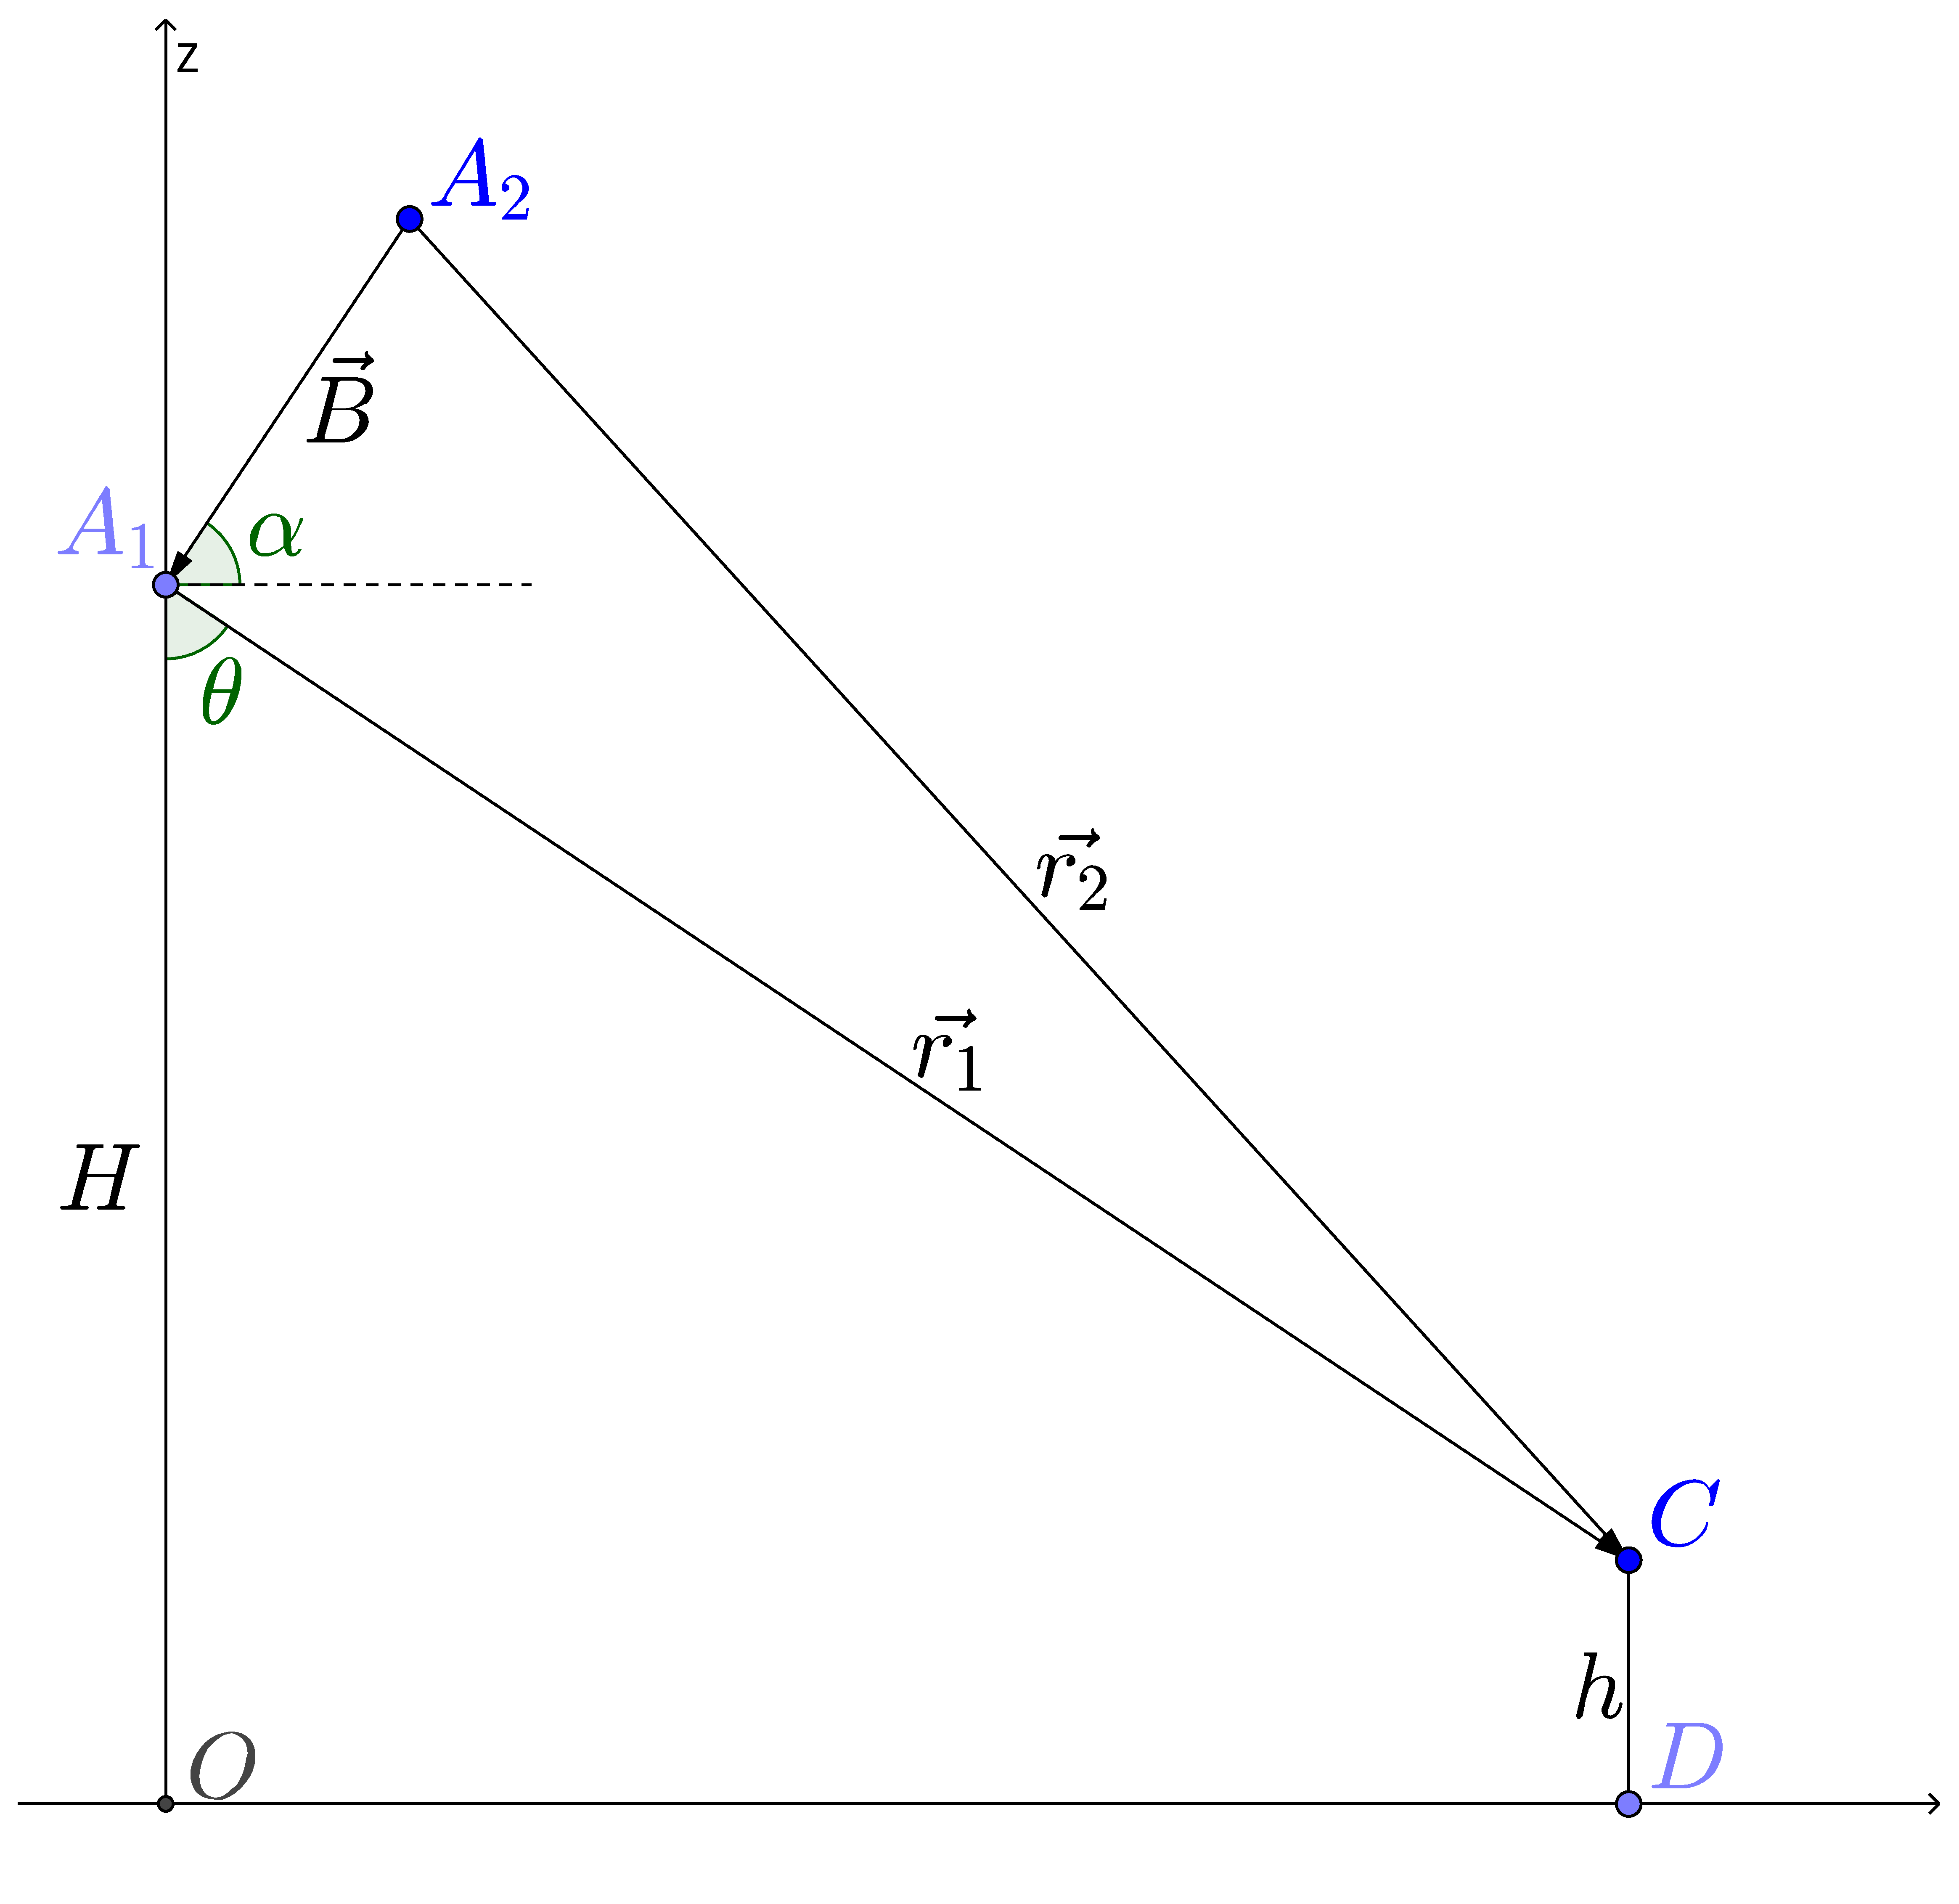
\includegraphics[width=0.4\textwidth]{insar_simple}
\caption{InSAR 高程测量基本原理} \label{fig:insar_simple}
\end{figure}

图 \ref{fig:insar_simple} 展示了利用两个 SAR 雷达观测同一地面单位进行 InSAR 测高的基本原理。InSAR 测量地表形变的原理与之类似。$A_1$ 和 $A_2$ 表示主天线和副天线位置,两天线空间位移矢量为 $\vec{B}$,称为 InSAR 基线,角度 $\alpha$ 为基线与水平面夹角。$C$ 为地面目标点,相对于两天线的位移矢量分别为 $\vec{r_1}$ 和 $\vec{r_2}$,称为斜距。角度 $\theta$ 为主天线观察方向与竖直方向的夹角,称为下视角。

斜距矢量 $ \vec{r_1} $ 和 $ \vec{r_2} $ 可以根据天线方向和微波信号双程旅行时得到;雷达位置或 SAR 卫星轨道,即基线 $\vec{B}$ 和天线高度 $H$,也可以认为是已知的。

由简单的几何关系可知,目标点高度可以表示为:

\begin{equation}
    h = H - r_1 \cos\theta
\end{equation}

为了得到 $\theta$,分别从主天线和副天线取得 SAR SLC 图像。目标点 $C$ 在两幅图像上的复像素值 $P_1$ 和 $P_2$ 可以表示为:

\begin{equation}
\begin{split}
    P_1(\vec{r_1}) = A_1(\vec{r_1}) \exp(i \frac{4\pi}{\lambda} r_1) \\
    P_2(\vec{r_2}) = A_2(\vec{r_2}) \exp(i \frac{4\pi}{\lambda} r_2) \\
\end{split}
\end{equation}

将两幅 SLC 图像共轭相乘,即得到一幅干涉图像:

\begin{equation}
    P_{\textrm{int}} = P_1^* P_2 =  A_1 A_2 \exp(i \frac{4\pi}{\lambda}(r_2 - r_1))
\end{equation}

干涉图相位项中的 $ r_2 - r_1 $ 可以通过余弦定理展开:
\begin{equation}
\begin{split}
    r_2 - r_1 &= r_1 (\frac{r_2}{r_1} - 1) \\
              &= r_1 \sqrt{1- \frac{\vec{r_1} \cdot \vec{B}}{r_1} + (\frac{B}{r_1})^2}
\end{split}
\end{equation}

基线长度 $B$ 一般远小于斜距 $r_1$、$r_2$,上式可以简化为:
\begin{equation}
    r_2 - r_1 = - \vec{r_1} \cdot \vec{B} = - r_1 B \cos(\frac{\pi}{2} - \theta + \alpha)
\end{equation}

故 $\theta$ 可以通过干涉图相位求出,进而得到目标点高程 $h$。然而,实际上回波相位(SAR 图像相位)是折叠到一个 $2\pi$ 周期内的,因此干涉图相位的值域也折叠在一个 $2\pi$ 周期中,这称为相位缠绕(phase wrap)。连续的相位值仍可以通过一些相位解缠算法估计出来。

实际使用 InSAR 测高时,还必须考虑地球曲率的影响。测量地表形变或位移时,原始地形引起的相位差也要通过数字高程模型去除。在过去,雷达轨道信息的精度也会影响 InSAR 成像精度;近些年,得益于卫星定位技术的发展,雷达轨道已经可以比较精确地获知。此外,电离层噪声、对流层噪声等因素也会影响 InSAR 成像的精度。

\subsection{InSAR 成像算法}

虽然 InSAR 测高原理非常简单,但实际的成像算法要复杂得多。主要可以归纳为以下若干步骤:

\textbf{SAR 成像和预处理}:相位差的测量精度决定了 InSAR 测高的精度。进行干涉的两幅 SAR 图像必须对成像区域有较好的聚焦,并且具有合适的基线长度,往往需要在若干组 SAR 数据中进行\textbf{筛选}。为了提取成像区域的有效信息,往往需要对 SAR 数据或者 SLC 图像进行\textbf{拼接}和\textbf{切割}。

\textbf{图像配准}:进行干涉成像之前,要通过图像配准将两幅 SAR 图像的像素精确对齐。SAR 图像像素大致对应于 SAR 雷达分辨率(数十米量级\cite{sandwell2011gmtsar})。虽然轨道数据已经可以较为精确地提供主副 SAR SLC 图像之间的偏移信息,但往往仍存在1~2个像素的误差\cite{sandwell2011gmtsar}。为了取得次像素级的配准精度,往往需要使用两幅图像的互相关特征进行修正。图像配准是成像程序中计算复杂度较高的一个步骤。

\textbf{干涉成像}:将对齐的主副 SAR SLC 图像进行共轭相乘,得到干涉图像。干涉图的相位被折叠到一个 $2\pi$ 周期上。根据上一节的推导,干涉图的相位信息反映了地面高程或地表位移信息。

\textbf{相位修正}:根据研究对象的不同,从干涉图中可选地去除地形相位、电离层延迟等不需要的相位项,以及滤除各种影响结果精度的噪声。

\textbf{相位解缠}:利用(一般情况下)高程或形变的连续性,从折叠相位恢复出连续变化的相位,以在较大的尺度上反映高程或形变信息。

上述步骤即为 InSAR 成像程序的主要功能。除此之外,包括 GMTSAR 在内的 InSAR 处理软件还支持地形图叠加等辅助分析功能,研究人员可以按需进一步处理。

\section{InSAR 成像算法 CPU 并行优化}

本节将以 GMTSAR 中图像拼接预处理和相位解缠两个程序模块为例子,介绍 CPU 并行的 InSAR 成像程序的算法设计和具体实现。

\subsection{并行图像配准算法设计}

GMTSAR 中主要由 xcorr 和 fitoffset.csh 程序实现图像配准。GMTSAR 将主 SAR SLC 图像像素到副 SLC 图像之间的映射近似为一个二维仿射变换,可以通过6个变换参数定义。主 SLC 图像的像素 $(x_i, y_i)$ 因为轨道偏移被映射到副 SLC 图像上的 $(x_i', y_i')$,两个坐标通过仿射变换矩阵相联系:

\begin{equation}
\begin{bmatrix}
  t_i x_i' \\
  t_i y_i' \\
  t_i \\
\end{bmatrix}
= \begin{bmatrix}
       a & b & c \\
       d & e & f \\
       0 & 0 & 1 \\
\end{bmatrix}
\begin{bmatrix}
  x \\
  y \\
  1 \\
\end{bmatrix}
\end{equation}

为了拟合6个仿射变换参数,xcorr 从主 SLC 图像中等间隔选取 $n_x \times n_y $ 个大小为 $x_s \times y_s$ 大小的采样窗口,与副 SLC 图像中对应的采样窗口通过 FFT 方法计算(散射系数幅度的)互相关,以估计该采样窗口处图像的偏移量。副 SLC 图像中对应采样窗口位置是通过卫星轨道参数估计的;如上一节所说,用卫星参数估计的偏移量误差在几个像素的量级。xcorr 中默认取 $n_x=64$ 和 $n_y=64$ 以保证采样窗口的相关性。fitoffsetsh 从 xcorr 输出中选择相关性较好的采样窗口,作为拟合仿射变换参数的数据点。

对于次像素级的图像配准处理,一般需要对原始数据或互相关矩阵进行插值处理,目前并没有一个公认的方法。不同论文选择的插值算法、插值顺序都有所区别\cite{li2008image}\cite{hanssen1999evaluation}。xcorr 在计算互相关矩阵前后分别进行了两次 sinc 插值(具体算法流程如图 \ref{fig:xcorr} 所示):

\begin{figure}[htbp]
\centering
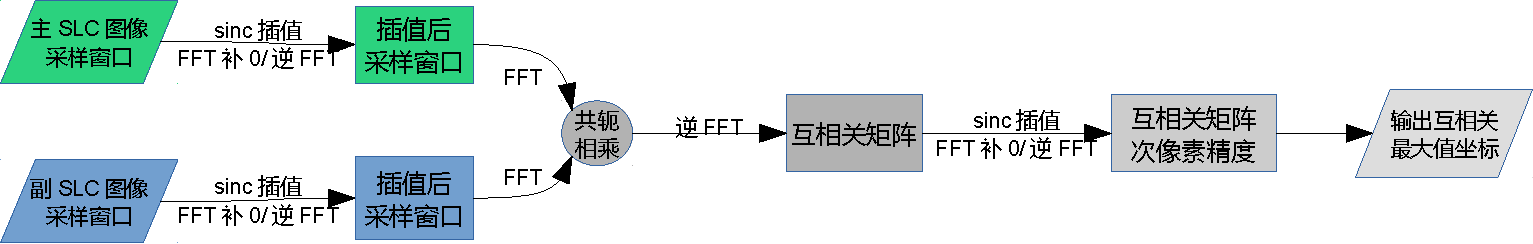
\includegraphics[width=0.99\textwidth]{xcorr-crop}
\caption{GMTSAR xcorr 采样窗口次像素配准流程} \label{fig:xcorr}
\end{figure}

\textbf{SLC 图像的距离向插值}:\citet{sandwell2011gmtsar} 指出,基于大地定位系统的卫星轨道数据所导致的 SLC 图像误差,在距离向更显著一些。为了弥补距离向较低的精度,在计算互相关矩阵前,xcorr 在距离向对 SLC 图像采样窗口的像素进行了 sinc 插值。sinc 插值可以通过 FFT 和频域补0高效地实现。插值因子默认为2。

\textbf{互相关矩阵插值}:对互相关矩阵插值并获得互相关峰值位置的坐标,是取得次像素偏移量的常用方法。一般采用线性插值、sinc 插值或者样条插值方法,理想情况下可以达到约0.1像素的配准精度\cite{li2008image}。这一步 xcorr 使用的仍是 sinc 插值,默认插值因子在方位向和距离向均为16。

上述配准流程算法仍有改进空间。图像配准实际上只用到复像素的幅度值(即 SAR 散射系数幅度)信息。除了距离向插值要使用复序列 FFT 对原始序列进行处理,后面的算法流程只需要处理时域实像素值,因此可以使用实序列 FFT 算法(FFT of real data,RFFT)处理采样窗口和互相关矩阵即可。处理实序列时,RFFT 比复序列 FFT 节省一半的运行时间和存储空间。改进后的配准流程如图 \ref{fig:xcorr2} 所示。


\begin{figure}[htbp]
\centering
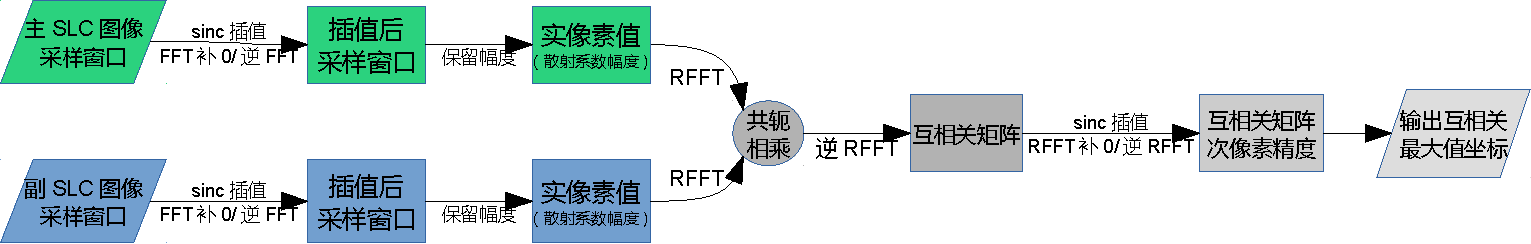
\includegraphics[width=0.99\textwidth]{xcorr2-crop}
\caption{改进的采样窗口次像素配准流程,部分复序列 FFT 算法改成了实序列 FFT 算法(RFFT)} \label{fig:xcorr2}
\end{figure}


本课题基于上述的 GMTSAR xcorr 模块的图像配准算法,设计了并行 SLC 图像配准程序 xcorr2。首先从计算复杂度、内存占用、文件读取三个角度定性分析 xcorr2 并行算法的预期性能指标:

\begin{itemize}
    \item \textbf{计算时间}:对于 $64 \times 64 = 4096$ 点的采样窗口,现代桌面 CPU 完成单线程复序列 FFT 计算的时间大约在几 ms 到 50ms 的数量级\cite{fftwbench}。经过实际测试,每个采样窗口的配准过程需要计算大约9次FFT变换或反变换。而以默认参数完成整幅图像配准需要遍历 512 个采样窗口。作为一个简单的估计,完成一次配准需要的 CPU 单线程计算时间约为 10~100s。
    \item \textbf{内存占用}:SAR SLC 图像文件大小可达数GB,但配准过程只需要读取采样窗口的数据。一个默认大小的采样窗口有 $64 \times 64 = 4096$ 个数据点,但插值后的互相关矩阵具有 $1024^2 = 1M$ 个数据点。考虑到计算过程要存储若干次中间结果,包括 FFT 变换结果、插值序列和互相关矩阵等,将数据点的数量乘以10作为估计值,即需要存储约 10M 个数据点,则可以估计每个采样窗口的配准过成需要的存储空间约为数十 MB。并行算法会增加内存开销(正比于计算线程数量),但相对于桌面工作站典型的 4~16GB 的内存配置,预期的内存占用并不大。
    \item \textbf{文件读取延迟}:典型的机械硬盘由于物理延迟则至少在 10ms 的量级\cite{wiki:hddcharacter},相比于 FFT 计算时间仍是不可忽略的。考虑使用单独的线程进行文件读取,并使用更多的内存预存 SLC 数据。
\end{itemize}

\begin{figure}[ht]
\centering
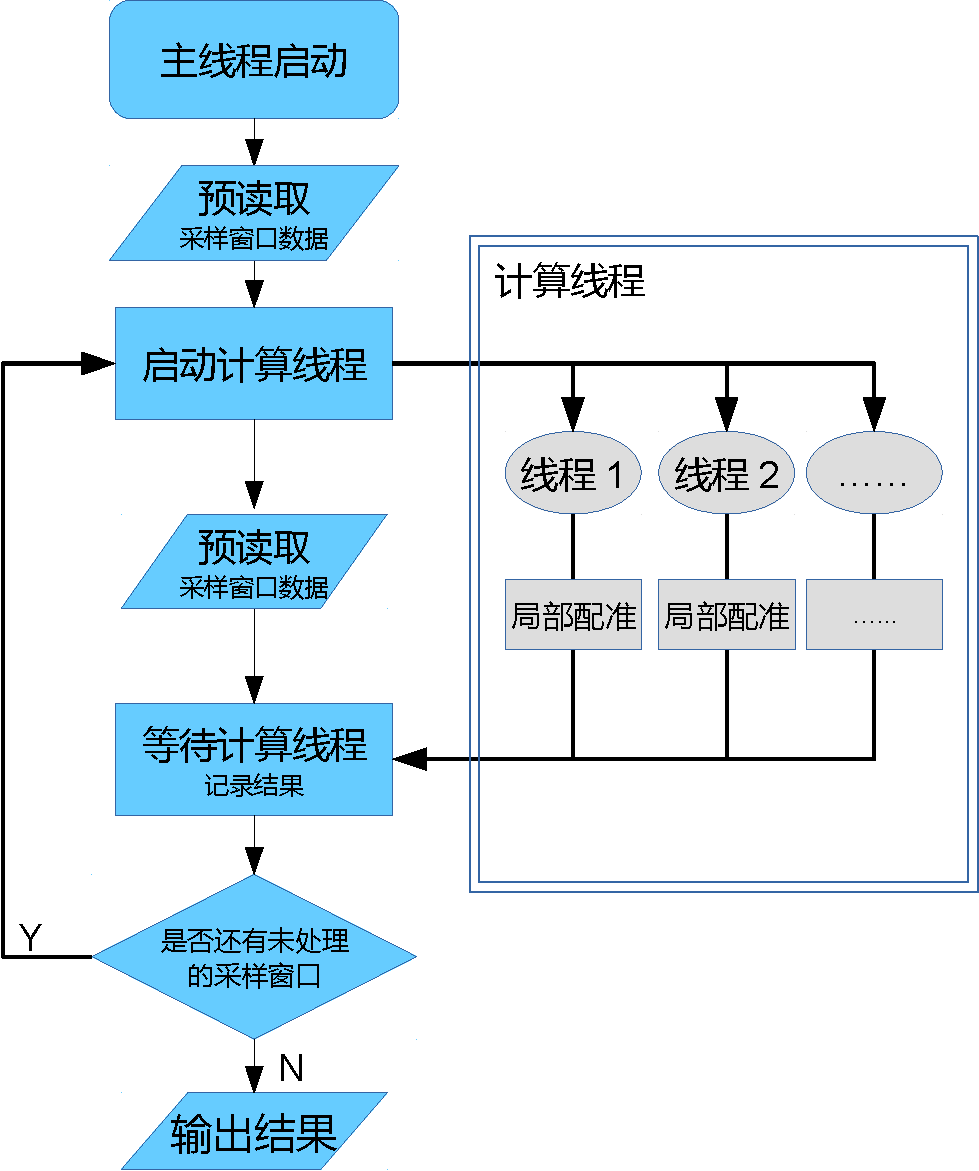
\includegraphics[width=0.6\textwidth]{parallel}
\caption{xcorr2 并行图像配准程序多线程架构(副线程计算流程同图\ref{fig:xcorr2})} \label{fig:parallel}
\end{figure}

综合上述因素,xcorr2 使用了如图\ref{fig:parallel}所示的主-副多线程并行架构。这一设计的核心是用独立的\textbf{主线程}进行数据预读取,而线程池中的\textbf{计算线程}则只执行计算操作。因为只有一个线程执行文件读取,可以充分发挥机械硬盘顺序读写的优势,不会因多线程文件读取相互竞争影响性能。内存开销方面,主线程每次只提前多读取一组待处理的采样窗口数据,并行内存开销相当于 单线程内存开销 $\times$ 线程数 $\times 2$。理想情况下,主线程文件读取操作与计算线程计算任务完全并行、并且文件读取不慢于单个采样窗口配准计算所需的时间(按照前面的分析应当是成立的),则并行算法的加速比应当正比于计算线程数量。


\subsection{并行图像拼接算法设计}

\subsection{其他程序模块的并行优化}
